\documentclass[11pt]{article}

% Language setting
% Replace `english' with e.g. `spanish' to change the document language
\usepackage[french]{babel}
\usepackage{braket}
\usepackage{amsfonts} 
\usepackage{subcaption}
\usepackage[T1]{fontenc}
% Set page size and margins
% Replace `letterpaper' with `a4paper' for UK/EU standard size
\usepackage[a4paper,top=2cm,bottom=2cm,left=3cm,right=3cm,marginparwidth=1.75cm]{geometry}

% Useful packages
\usepackage{amsmath}
\usepackage{graphicx}
\usepackage[colorlinks=true, allcolors=black]{hyperref}

\title{\textbf{Etude de la Mesure Quantique, Application à l'Effet Zénon}}
\author{Théo HUET}
\date{}

\begin{document}

\begin{figure}[h]

\includegraphics[scale=0.6]{cy.jpg}
\vspace{6cm}

\maketitle
\end{figure}
\thispagestyle{empty}
\vspace{8.6cm}

\centering
Stage de 3ème année Licence de Physique
\\
Effectué au \href{https://www.cyu.fr/recherche-et-valorisation/structures-de-recherche/laboratoires/laboratoire-de-physique-theorique-et-modelisation}{\textbf{laboratoire de Physique Théorique et Modélisation}}
\\
à CY Cergy Paris Université \\
du 29 avril 2024 au 29 mai 2024
\begin{center}
    Sous la direction de Monsieur \href{https://www.cyu.fr/lorenzo-fratino}{\textbf{L. Fratino}}
    \\
    Enseignents-chercheurs\\
    \textit{lorenzo.fratino@u-cergy.fr}
\end{center}




\newpage
\thispagestyle{empty}
\raggedright
\tableofcontents\text{}

\newpage

\setcounter{page}{1}
\section{Introduction}

\qquad Ce stage sur l'effet Zénon quantique a été réalisé en fin de licence sous la supervision de Monsieur Fratino, enseignant-chercheur en physique au Laboratoire de Physique Théorique et Modélisation (LPTM) de CY Cergy Paris Université. 
\\Le LPTM se distingue par ses recherches approfondies en physique théorique, qui mettent l'accent sur la physique statistique des grands systèmes à des énergies "basses". Ces travaux requièrent une combinaison de méthodes mathématiques et numériques et couvrent un large éventail de domaines, notamment la modélisation des systèmes de matière condensée, des systèmes physiques non linéaires, des systèmes intégrables, des systèmes complexes, des systèmes biologiques et des systèmes "actifs".\\
\vspace{0.5cm}
\qquad Mon objectif au cours de ce stage est d'approfondir mes connaissances en physique quantique acquises au cours des deux dernières années, en me concentrant spécifiquement sur l'étude de l'effet Zénon et de la mesure, à la fois par des calculs purement théoriques et l'analyse de résultats expérimentaux.\\
\vspace{0.5cm}
\qquad L'effet Zénon, nommé d'après le philosophe grec Zénon d'Élée, est un phénomène fascinant découlant des principes de la mécanique quantique. Il évoque l'idée que l'observation répétée d'un système quantique par un appareil de mesure peut bloquer son évolution ou son mouvement, cette notion fondamentale trouve notament des applications importantes dans le domaine de l'informatique quantique, domaine qui m'attire particulièrement pour mes futures orientations de recherche.\\
\vspace{0.5cm}
\qquad Ce concept a été proposé pour la première fois en 1977 par Georges Sudarshan et Baidyanath Misra. Bien que la paternité théorique de l'effet Zénon soit souvent attribuée à Alan Turing également, il a fallu attendre 1989 pour qu'il soit observé expérimentalement, grâce à l'utilisation d'ions refroidis par laser et piégés par des champs magnétiques et électriques.



\newpage

\section{Les Postulats de la Physique Quantique}

\qquad Nous allons tout d'abord, pour mieux comprendre notre sujet, revenir aux bases de la Physique Quantique et principalement sur celles liées à la mesure. Voyons donc les Postulats de la mécanique quantique~\cite{wikPM}.

\subsection{Postulat I : L'état d’un système}

L'état d'un système quantique est complètement contenu, à l'instant \( t \), dans un vecteur normalisable \( \ket{\psi} \in H \), un espace de Hilbert.

\subsubsection{Normalisation}

Normaliser un état signifie que \( \braket{\psi|\psi} = 1 \). La condition de normalisation correspond à l’exigence selon laquelle les probabilités de tous les résultats possibles d’une mesure quantique sont \( 1 \).

\subsubsection{États Orthogonaux}

Des états sont dits orthogonaux entre eux mathématiquement si l'on a \( \braket{\psi|\phi} = 0 \).
Physiquement, on peut qualifier des états orthogonaux comme étant des états incompatibles classiquement, comme par exemple :
\vspace{0.3cm}
\begin{itemize}
\renewcommand{\labelitemi}{$\cdot$}
    \item Une pièce de monnaie ne peut pas être à la fois sur pile et face.
    \item Le chat de Schrödinger ne peut pas être à la fois vivant et mort.
\end{itemize}

\subsubsection{La Superposition d'États}

En Quantique, toute combinaison linéaire d'états orthogonaux une fois normalisée peut être un état du système, donc il est possible d'avoir un état qui est dit "superposé".
\vspace{0.5cm}

Donc le chat de Schrödinger peut être dans l'état \( \ket{\psi} = \frac{\ket{vivant} + \ket{mort}}{\sqrt{2}} \) (voir figure 1).

\begin{figure}[h]
 \caption{Exemple de Superposition avec le chat de Schrödinger dans sa boîte~\cite{figure}}
 \vspace{0.5cm}
 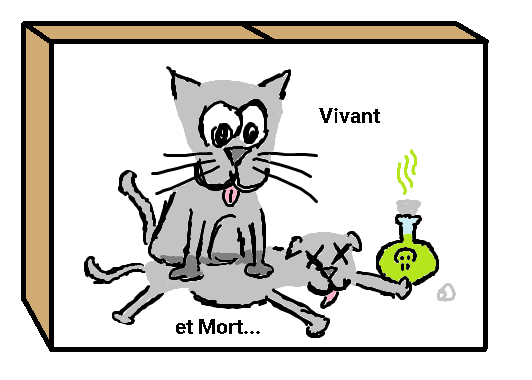
\includegraphics[scale=0.6]{postulat 1 chat.png}
 \centering
 \label{fig:superposition}
\end{figure}

\subsection{Postulat II : Les observables}

\qquad Toute propriété observable comme la position ou l'énergie correspond à un opérateur, comme par exemple \( \hat{A} \), hermitien linéaire agissant sur les vecteurs d'état \( \ket{\psi} \). Cet opérateur est nommé observable.


 \newpage
 
\subsection{Postulat III : Résultat d'une mesure}

La mesure d'une grandeur physique représentée par l'observable \( \hat{A} \), que l'on nomme opérateur, va nous donner comme résultat l'une des valeurs propres de \( \hat{A} \), que l'on note \( \lambda_n \). Les vecteurs propres \( \ket{\lambda_n} \) associés aux valeurs propres seront l'état quantique du système immédiatement après la mesure (voir figure 2).\\
On peut écrire ce postulat en notation braket que l'on utilisera pour la suite :
\[
\hat{A} \ket{\lambda_n} = \lambda_n \ket{\lambda_n}
\]

\begin{figure}[h]
 \caption{Mesure d'un état \( \ket{\psi} \) par l'observable \( \hat{A} \)~\cite{figure}}
 \vspace{0.5cm}
 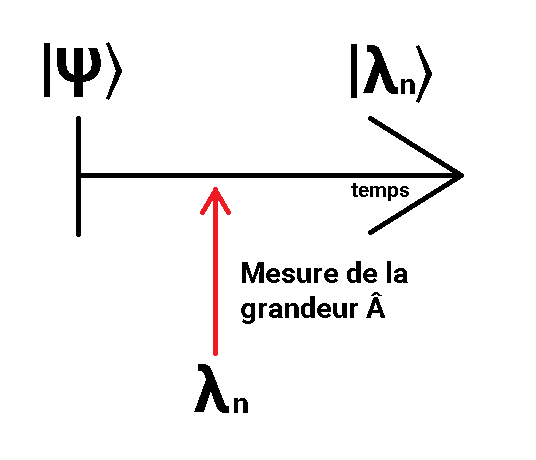
\includegraphics[scale=0.4]{postulat 3.png}
 \centering
 \label{fig:mesure}
\end{figure}

Remarque importante : Tout état peut se décomposer dans une base \( (\ket{\lambda_n})_{n} \) formée par les vecteurs propres qui sont orthogonaux entre eux (si les valeurs porpres ne sont pas degenerées), de n'importe quel observable. Ainsi, cette base est orthonormale et permet de décrire n'importe quel état.

\subsection{Postulat IV : Règle de Born}

On a vu que les \( (\ket{\lambda_n})_n \) sont les états possibles après une mesure. \\
La probabilité d'avoir l'état \( \ket{\lambda_n} \) et de mesurer \( \lambda_n \) après l'application d'un opérateur \( \hat{A} \) sur un état \( \ket{\psi} \) est :
\[
p_n = |\braket{\lambda_n|\hat{A}|\psi}|^2
\]
On appelle cela la règle de Born.

\begin{figure}[h]
 \caption{Arbre de Probabilité des états après une mesure de \( \hat{A} \)~\cite{figure}}
 \vspace{0.5cm}
 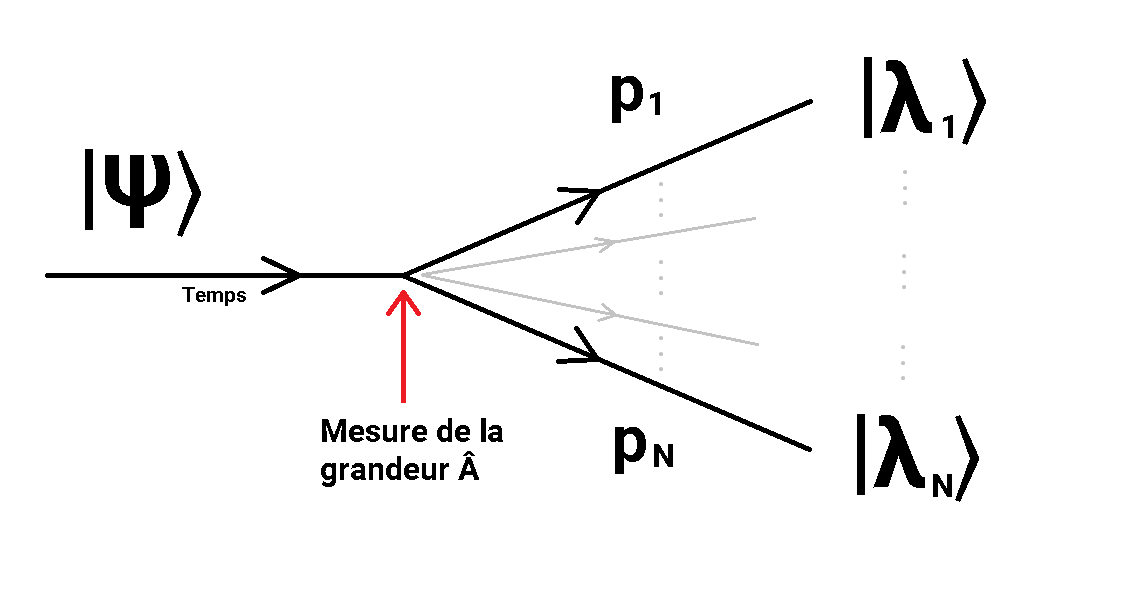
\includegraphics[scale=0.3]{postulat 4.png}
 \centering
 \label{fig:probabilite}
\end{figure}


 \newpage 
 
\subsection{Postulat V : Réduction du paquet d'onde} \label{sec:PV}

Ce postulat est en lien avec le précédent. Il nous dit que l'état après la mesure, que l'on note \( \ket{\psi_{\text{final}}} \) si l'on mesure la valeur \( \lambda_n \), est donné par :
\[
\ket{\psi_{\text{final}}} = \frac{\hat{P} \ket{\psi}}{\sqrt{p_n}}
\]
avec \( \hat{P} \) le \hyperref[sec:Projecteur]{\texttt{projecteur}} des vecteurs propres associés à la valeur propre \( \lambda_n \).
On a donc un écrasement de la fonction d'onde, une réduction du paquet d'onde~\cite{wikRED} (voir figure 4).

\qquad En effet, une fois mesuré, notre système va se mettre dans l'état mesuré. Ainsi, on perd toute superposition d'état.

\qquad C'est l'un des concepts les plus compliqués à comprendre avec la superposition d'un point de vue logique, basé sur la physique classique. Cependant, cela a été prouvé de nombreuses fois expérimentalement, comme avec l'expérience des fentes de Young.
\qquad C'est ce phénomène qui a lieu dans l'expérience du chat de Schrödinger : le chat sera à la fois mort et vivant dans la boîte (voir figure 1), et une fois ouverte, il sera soit mort, soit vivant, mais pas les deux. L'état du système est réduit à un seul état et perd sa superposition une fois la boîte ouverte, synonyme de mesure.

\begin{figure}[h]
 \caption{Exemple de Réduction de la fonction d'onde \( \psi(t,x,y,z) \)~\cite{figure}}
 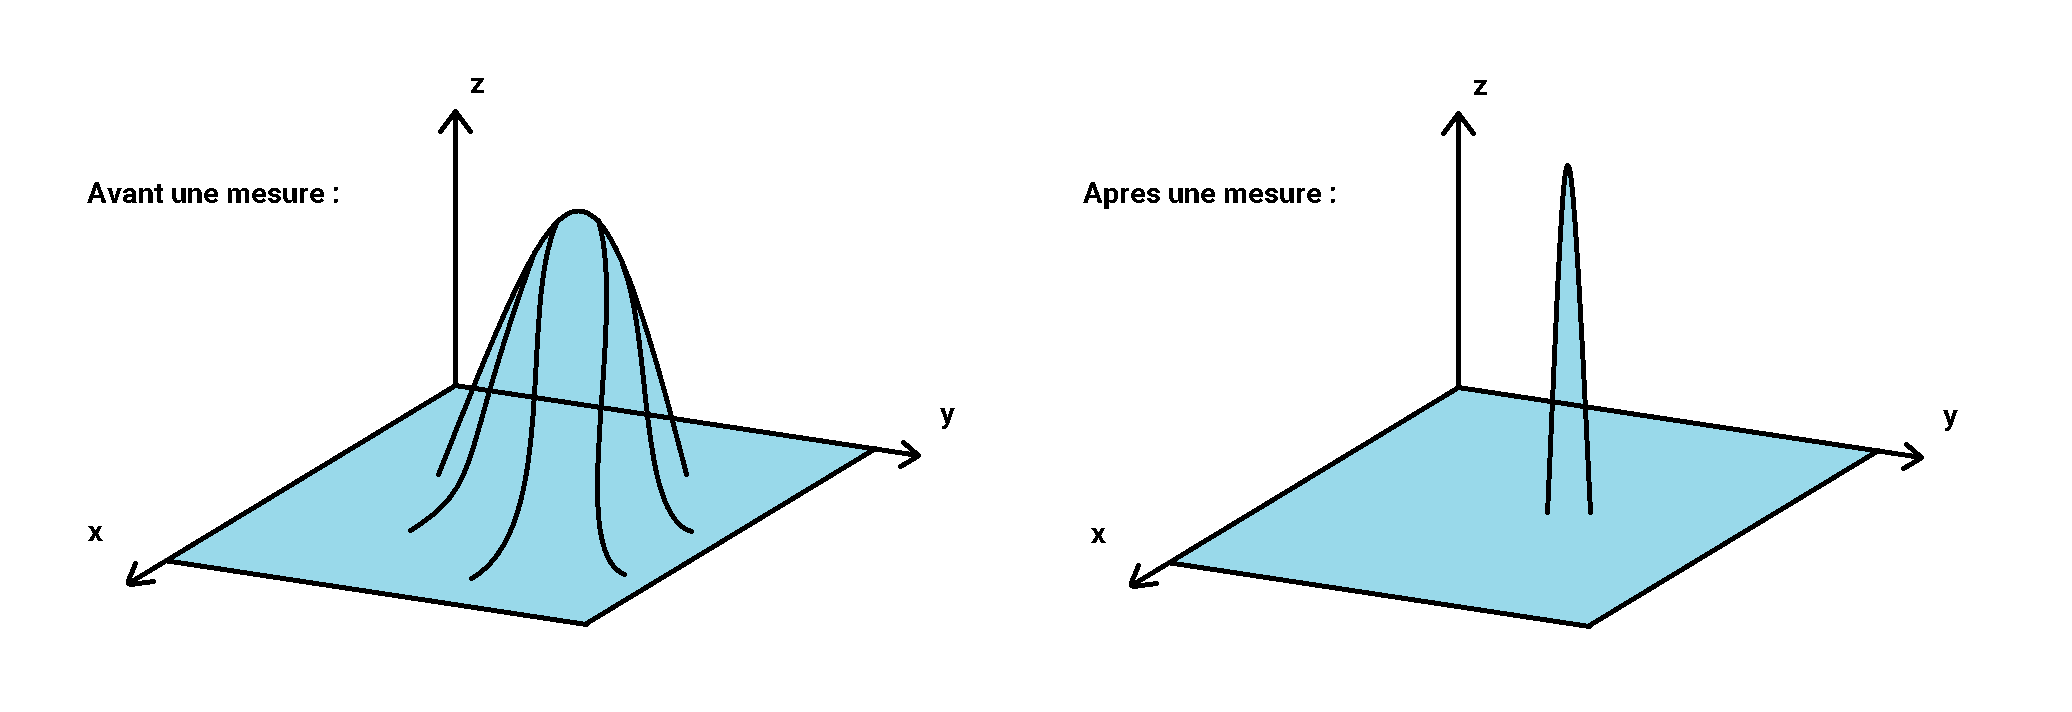
\includegraphics[scale=0.3]{postulat 5.png}
 \centering
 \label{fig:reduction}
\end{figure}

Pour essayer de comprendre ce phénomène, on peut utiliser la théorie de la décohérence~\cite{wikDQ} ou bien l'interprétation de Coleman sur la mesure~\cite{ColemanInt}.

\subsection{Postulat VI : Équation de Schrödinger}

Le dernier postulat concerne l'équation de Schrödinger. En effet, chaque état doit être solution de l'équation :
\[
i\hbar \frac{\partial}{\partial t} \ket{\psi} = \hat{H} \ket{\psi}
\]
avec \( \hat{H} \) l'opérateur Hamiltonien qui est donc responsable de l'évolution du système dans le temps.

\subsubsection{L'opérateur évolution temporelle}

On le note \( \hat{U}(t) \). Il permet de décrire le système à un temps \( t \) en ayant connaissance de l'état du système au temps \( t=0 \), que l'on note \( \ket{\psi_0} \).
Ainsi, on a par définition :
\[
\ket{\psi(t)} = \hat{U}(t) \ket{\psi_0}
\]
Comme \( \ket{\psi(t)} \) suit l'équation de Schrödinger, si on pose \( \hat{H} \) constant par rapport au temps, on obtient :
\[
\hat{U}(t) = e^{\frac{\hat{H} t}{i\hbar}}
\]


\newpage

\section{Mesure Quantique}
\qquad Nous pouvons maintenant regarder plus en détail la mesure en physique quantique qui va avoir un effet très important pour la suite.
Nous savons que la mesure impacte le système mesuré de façon irréversible (réduction du paquet d'onde), mais comment peut-on maîtriser cela ?\\
\qquad Les mesures quantiques peuvent être différenciées en deux catégories : les mesures fortes et les mesures faibles~\cite{wikF}, qui ont toutes les deux leurs spécificités. 

\subsection{Mesure Forte ou de von Neumann}
\qquad La mesure forte est, en quelque sorte, la mesure à laquelle on pense tout de suite si l'on souhaite mesurer une grandeur. Elle permet en effet de déterminer la valeur d'une grandeur physique.\\
\qquad Sa limite est qu'elle induit un effondrement complet de la fonction d'onde, donc une réduction du paquet d'onde. Cela donne alors un résultat précis sur ce que l'on veut mesurer, cepandant l'état du système est entièrement réduit à celui qui a été mesuré, comme nous l'indique le \hyperref[sec:PV]{\texttt{Postulat V}} : on perd la superposition d'état s'il y en a une.

\subsection{Mesure Faible}
\qquad Pour éviter cela et donc garder un état superposé, on peut utiliser un autre type de mesure qui, cette fois-ci, nous donne des résultats dépourvus de sens physique immédiat.
La mesure faible perturbe donc le système de manière minimale, ainsi on peut conserver une superposition permettant une analyse sans altérer sa dynamique. Cela permet, par exemple, de garder un couple de particules intriquées (EPR), très utile en télécommunications quantiques. %faire un exemple de Bell qui est conservé

\subsection{Exemples de mesure forte et faible}
Soient : \\
\begin{itemize}
\renewcommand{\labelitemi}{$\cdot$}
    \item \( \sigma_x = \)
    \( \begin{pmatrix}
    0 & 1 \\
    1 & 0
    \end{pmatrix} \) avec \( \ket{\rightarrow} \) le vecteur propre associé à la valeur propre \( \lambda_{\ket{\rightarrow}} = 1 \) et \( \ket{\leftarrow} \) le vecteur propre associé à la valeur propre \( \lambda_{\ket{\leftarrow}} = -1 \) \\
    \item \( \sigma_z = \)
    \( \begin{pmatrix}
    1 & 0 \\
    0 & -1
    \end{pmatrix} \) avec \( \ket{\uparrow} \) le vecteur propre associé à la valeur propre \( \lambda_{\ket{\uparrow}} = 1 \) et \( \ket{\downarrow} \) le vecteur propre associé à la valeur propre \( \lambda_{\ket{\downarrow}} = -1 \) \\
\end{itemize}
les Matrices de Pauli
 \begin{tabbing}
    on pose \( \ket{\psi} = \ket{\rightarrow} = \frac{\ket{\uparrow} + \ket{\downarrow}}{\sqrt{2}} \)
    
\end{tabbing}

\begin{tabbing}
    alors \( \sigma_x \ket{\psi} = \sigma_x \ket{\rightarrow} = \ket{\rightarrow} = \frac{\ket{\uparrow} + \ket{\downarrow}}{\sqrt{2}} \)
\end{tabbing}
\( \ket{\rightarrow} \) est un vecteur propre de \( \sigma_x \), donc après notre opération de mesure, on conserve la superposition des spins up et down. Nous avons donc effectué une mesure faible sur le spin up et down.
\begin{tabbing}
    et on a \( \sigma_z \ket{\psi} = \sigma_z \frac{\ket{\uparrow} + \ket{\downarrow}}{\sqrt{2}} = \frac{\ket{\uparrow} - \ket{\downarrow}}{\sqrt{2}} \) 
\end{tabbing}

\( \ket{\uparrow} \) et \( \ket{\downarrow} \) sont tous les deux des vecteurs propres de \( \sigma_z \), donc après notre mesure, deux résultats sont possibles et tous deux ne sont pas des états superposés du spin up et down.
\\Donc en appliquant \( \sigma_z \), on obtient que notre système devient un état non superposé. Il s'agit d'une mesure forte sur le spin up et down.


\newpage

\section{Effet Zénon}
\qquad L'effet Zénon a pour but de décrire le fait qu'en mesurant en "continu" un objet, l'état de celui-ci n'évolue pas. Cela pourrait potentiellement permettre au chat de Schrödinger de rester en vie avant que l'on vienne ouvrir la boîte.\\
\qquad Nous allons donc voir comment c'est possible avec des raisonnements théoriques et expérimentaux.

\subsection{Cas simple : l'Hamiltonien est indépendant du temps}
L'opérateur \hyperref[sec:Projecteur]{\texttt{Projecteur}} $\hat P = \ket{\psi_0}\bra{\psi_0}$ a deux valeurs propres $\lambda_1 = 1$ associées au vecteur propre $\ket{\psi_0}$ et $\lambda_0 = 0$ associée au vecteur propre $\ket{\lambda_0}$.

Si l'on cherche la probabilité d'avoir l'état $\ket{\psi_0}$ après la mesure au temps $t$, on a :
\[ \text{proba}(t) = | \braket{\psi_0|\hat P|\psi(t)} |^2 \] d'après Born.\\
Ici, $\ket{\psi(t)} = \hat U(t)\ket{\psi_0}$, et l'Hamiltonien ne dépend pas du temps, donc l'opérateur évolution est :
\[ \hat U(t) = e^{\frac{\hat H t}{i\hbar}} = \sum_{i=0}^{+\infty} (\frac{\hat H t}{i\hbar})^n \frac{1}{n!} \approx 1 + \frac{\hat H t}{i\hbar} - \frac{\hat H^2t^2}{2\hbar^2} + O(t^3) \]
On peut faire un DL en 0 car le temps entre les mesures va etre suppopsé court, le système aura peu de temps pour évoluer donc $1 \gg t$.\\
\vspace{0.2cm}
Ainsi, \qquad $p_1(t) = |\braket{\psi_0|\hat P|\hat U(t)|\psi_0}|^2$ \qquad et \qquad $p_0(t) = 1 - p_1(t)$.\\
\vspace{0.2cm}
Or on a $\hat P\ket{\psi_0} = \ket{\psi_0}$, donc
\[ p_1(t) = |\braket{\psi_0|\hat U(t)|\psi_0}|^2 \approx |1 + \frac{\braket{\hat H}t}{i\hbar} - \frac{\braket{\hat H^2}t^2}{2\hbar^2}|^2 \approx 1 - \frac{\Delta \hat H^2 t^2}{\hbar^2} + O(t^4) \]
Car on a la valeur moyenne d'un opérateur quelconque $\hat A$ dans un système d'état $\ket{\psi}$ qui est $\braket{A} = \braket{\psi|\hat A|\psi}$,\\
et par définition on a $\Delta \hat H^2 = \braket{\hat H^2} - \braket{\hat H}^2$.\\
\vspace{0.5cm}
De plus, $p_1(t) \equiv p(t|0)$, c'est-à-dire la probabilité que l'état $\psi(t) = \psi_0$ après la mesure au temps $t$, sachant que $\psi(t=0) = \psi_0$.\\
\vspace{0.3cm}
Si on trouve donc la valeur 1 au temps $t_1$, alors $p(t_2|t_1) = p_1(t_2-t_1)$ pour tout $t_2 > t_1$ car on est dans le même cas que pour $t_1 = 0$.

On a donc
\[ p(t_2|t_1) \simeq 1 - \frac{\Delta^2 \hat H}{\hbar^2}(t_2 - t_1)^2 \]
Et comme on a supposé que $\hat H$, l'Hamiltonien, ne dépend pas du temps, \\
si l'on effectue maintenant une série de $N$ mesures de $P_0$ à des temps successifs équidistants $\Delta t$, on va avoir $t_n = n \Delta t$ avec $\Delta t = \frac{t}{N}$ et $t$ et $N$ (assez grand) fixés de telle sorte que $\Delta t$ soit assez petit.\\
\vspace{0.3cm}
On a donc comme probabilité, qu'à toutes les mesures, on trouve 1 :
\[ p_{pos} = p(t_N|t_{N-1}) \cdot p(t_{N-1}|t_{N-2}) \cdot ... \cdot p(t_2|t_1) \]
\[ \simeq \left(1 - \frac{\Delta^2 \hat H}{\hbar^2}\Delta t^2\right)^N = e^{N \ln\left(1 - \frac{\Delta \hat H^2 t^2}{\hbar^2N^2}\right)} \simeq e^{-\frac{\Delta \hat H^2 t^2}{\hbar^2N}} \xrightarrow[N \rightarrow +\infty]{} 1 \]

Donc, si l'on mesure en "continu" notre système, il n'évolue pas. En effet, la probabilité de trouver l'état initial à la fin du temps $t$ est de 1, c'est l'effet Zénon.

\newpage

\subsection{Cas particulier : Proposition de Cook}

\qquad Nous avons également Cook~\cite{cook} qui nous donne une proposition pour démontrer l'existence de l'effet Zénon. \\
Cook propose de prendre un atome à trois niveaux d'énergie, notés $\ket{1}$, $\ket{2}$, $\ket{3}$,\\
où le niveau $\ket{1}$ représente l'état fondamental, le niveau $\ket{2}$ est un état métastable avec une désintégration $2 \rightarrow 1$ négligeable, c'est-à-dire que pour redescendre il n'émet rien, et le niveau $\ket{3}$ est un niveau excité ordinaire, avec une durée de vie courte, $10^{-10}$ s.\\
Il est couplé exclusivement au fondamental $\ket{1}$, pour y accéder, il faudrait donc une impulsion optique de bonne énergie lorsque l'état est $\ket{1}$ (voir figure 5).\\
\vspace{0.5cm}
\qquad Dans le cas d'un ion piégé, les niveaux peuvent être manipulés facilement avec des champs de radiofréquences et des pulsations optiques.\\
La proposition va donc être de solliciter le couple $(\ket{1}, \ket{2})$ avec une excitation résonante de pulsation $\omega$ qui participe à l'oscillation de Rabi.\\
\qquad Les oscillations de Rabi désignent les transitions périodiques entre les états quantiques d'un système à deux niveaux, induites par l'interaction avec un champ électromagnétique oscillant à une fréquence proche de la résonance. Ces transitions peuvent se manifester par des oscillations entre les états individuels du système, ainsi que par la formation de superpositions quantiques entre ces états.\\
La transition $1 \leftrightarrow 2$ a besoin d'une pulsation $\omega_{0} = \frac{E_2 - E_1}{\hbar}$, de l'ordre de quelques centaines de MHz.\\
L'oscillation de Rabi se produit à une pulsation $\Omega$ de l'ordre de quelques dizaines de Hertz. On a donc $\omega_{0} \gg \Omega$ que l'on pourra utiliser plus tard.\\
\vspace{0.3cm}
Avec l'oscillation de Rabi, le troisième état $\ket{3}$ n'est pas accessible. Pour l'atteindre, il faudrait donc faire une impulsion optique de bonne énergie.\\
\vspace{0.5cm}
\qquad La suite du raisonnement est : en envoyant une impulsion optique, si l'état du système est $\ket{1}$, nous allons avoir une excitation jusqu'à l'état $\ket{3}$, celui-ci va se désexciter en émettant un photon (et donc retourner à l'état $\ket{1}$).\\
En revanche, si au moment de l'impulsion l'état du système est $\ket{2}$, le photon ne sera pas absorbé, il ne se passera rien.\\
Le but est donc de voir si en mesurant (envoyant une impulsion optique) en continu (ou avec un intervalle assez petit) l'état du système ne varie pas.
\vspace{0.5cm}
\begin{figure}[h]
 \caption{\label{étiquette} Diagramme des niveaux d'énergie que Cook propose pour démontrer l'effet Zénon~\cite{figure}}
 \includegraphics[scale=0.4]{3niveau d'énergie.png}
 \centering
 \end{figure}

\newpage

\subsubsection{Opérateur densité $\rho $}

Avant de voir la suite, il faut tout d'abord introduire un nouvel opérateur, l'opérateur densité, très en lien avec le projecteur dans le cas d'un état "pur" mais différent pour les états "mixtes".

\begin{itemize}
    \renewcommand{\labelitemi}{$\cdot$}
    \item État pur : dans ce cas, on connaît tout du système, tout est dans $\ket{\psi}$, l'entropie $S$ (ou le manque d'information) est donc nulle.
    \item État mixte : c'est un mélange statistique d'états purs. Il est de la forme $\sum_i c_i \ket{\psi_i}\bra{\psi_i}$.
\end{itemize}
\vspace{0.2cm}
L'opérateur densité va donc nous permettre de décrire notre système dans ces deux cas.\\
\vspace{0.3cm}
\qquad Soit $S$ un système entouré d'un thermostat à température $T$. Les probabilités de Boltzmann $P_n(\beta) \propto e^{-\beta E_n}$ sont les probabilités de trouver notre système dans un état d'énergie $E_n$, donc $\ket{E_n}$.\\
\vspace{0.2cm}
Avec $\beta = \frac{1}{k_B T}$ par définition.\\
\vspace{0.3cm}
Nous allons poser comme définition :

\[
\rho(\beta) = \frac{1}{Z(\beta)} e^{-\beta \hat H}
\]
avec $Z(\beta) = \sum_n e^{-\beta E_n}$ la constante de normalisation.\\
\vspace{0.2cm}
$\hat H$ dans la base $\ket{E_n}$ est diagonalisé avec comme diagonale les $E_n$, donc :

\[
\rho(\beta) = \frac{1}{Z(\beta)} \sum_n  e^{-\beta E_n}\ket{E_n}\bra{E_n} \equiv  \sum_n \rho_{nn}\ket{E_n}\bra{E_n}
\]

Avec les $\rho_{nn}$ tels que $\rho(\beta) = \begin{pmatrix}
    \rho_{11} & \cdots & 0\\
    \vdots & \ddots & \vdots\\
    0  & \cdots & \rho_{NN}\\
\end{pmatrix}$ est diagonale, dans un cas pur. 
\vspace{0.2cm}
Après une mesure, on sera forcément dans ce cas-là.\\
\vspace{0.5cm}
\qquad Maintenant, si on laisse passer le temps, notre système va évoluer et devenir mixte. On aura une matrice de la forme :
\vspace{0.2cm}

\qquad $\rho(\beta) = \begin{pmatrix}
    \rho_{11} & \cdots & \rho_{1N}\\
    \vdots & \ddots & \vdots\\
    \rho_{N1}  & \cdots & \rho_{NN}\\
\end{pmatrix}$ Elle n'est pas forcément diagonale.\\
\vspace{0.2cm}
Nous pouvons également écrire l'opérateur densité avec n'importe quelle base d'observable $\hat A$ avec $\hat A \ket{a_n} = a_n \ket{a_n}$, il s'agit d'une définition :

\[
\rho = \sum_n \rho_{nn}\ket{a_n}\bra{a_n} \Leftrightarrow Proba(A \rightarrow a_n) = P_n = \rho_{nn}
\]

En plus d'être diagonale, si le système est dans un état pur, nous avons :

\[
\text{pur} \Leftrightarrow S = 0 \Leftrightarrow \exists \ket{\psi} \text{ tels que } \rho = \ket{\psi}\bra{\psi} \Leftrightarrow \rho = \rho^2 \Leftrightarrow \rho \text{ est un projecteur}
\]

Nous aurons également $\ket{\psi} = \sum_n c_n\ket{a_n} \Rightarrow \rho = \sum_n c_n c_n^\ast \ket{a_n}\bra{a_n} \Rightarrow \rho_{nm} = c_n c_m^\ast$. \\
Si $n=m$, nous avons $|c_n|^2 = P_n$ que l'on connaît déjà.\\
\vspace{0.2cm}
Dans un cas où notre système peut naturellement être dans seulement deux états, comme ici l'état 1 et 2, nous avons $\rho$ qui est une matrice $2 \times 2$. \\
\vspace{0.2cm}
Nous savons que la somme des probabilités $= 1$, donc $P_1 + P_2 = 1 = \rho_{11} + \rho_{22} = Tr(\rho)$. \\
$\rho$ possède donc 3 degrés de liberté ($\rho_{11},\rho_{12},\rho_{21}$ car $\rho_{22} = 1 - \rho_{11}$), nous pouvons donc poser un vecteur $\Vec{R} \in \mathbb{R}^3$ qui décrit notre système.


\newpage

\subsubsection{{Les Projecteurs\texttt{}} \label{sec:Projecteur} }
\qquad Petit rappel, une mesure très importante en quantique est celle réalisée par un projecteur. Il s'agit de l'opérateur densité dans le cas pur, il va permettre à un état d'être projeté dans l'état qui compose le projecteur, \\
et nous permet de savoir si un système est dans un certain état bien particulier. \\
On le note $\hat P$, il se construit de la sorte que $\hat P = \hat P^2$.\\
En physique quantique, on pose le projecteur d'un état $\ket{\psi}$ comme $\hat P = \ket{\psi}\bra{\psi}$, \\
où l'on a bien $\hat P^2 = \ket{\psi}\braket{\psi|\psi}\bra{\psi} = \ket{\psi}\bra{\psi} = \hat P $.\\
\vspace{0.2cm}
Mathématiquement, on trouve 2 valeurs propres, $\lambda_1 = 1$ et $\lambda_0 = 0$. \\
\vspace{0.2cm}
En effet, on a $\hat P \ket{\phi} = \ket{\psi}\braket{\psi|\phi}$. 
\begin{itemize}
    \renewcommand{\labelitemi}{$\cdot$}
        \item Si $\ket{\phi} = \ket{\psi}$, \\
        alors $\braket{\psi|\phi} = 1$, donc $\hat P \ket{\psi} =\ket{\psi}$, $\ket{\psi}$ est un vecteur propre de $\hat P$ associé à la valeur propre $\lambda_1 = 1$.
        \item Si $\ket{\phi} \perp \ket{\psi}$,\\ 
        alors $\braket{\psi|\phi} = 0$, donc $\hat P \ket{\phi} = 0 \ket{\phi}$, $\ket{\phi}$ est un vecteur propre de $\hat P$ associé à la valeur propre $\lambda_0 = 0$. \\
        Remarque : \\
        $\lambda_0$ peut être dégénéré car il peut y avoir plusieurs états orthonormaux à $\ket{\psi}$.
    \end{itemize}
    
\subsubsection{Vecteur de Bloch $\Vec{R}$}

Nous avons également besoin de définir : \qquad $\Vec{R} = \begin{pmatrix}
    R_x\\R_y\\R_z
\end{pmatrix}$, \\
le vecteur qui indique le point de la sphère de Bloch (voir figure 6) correspondant à un état mixte donné. \\
Par conséquent, la surface de la Sphère (de Bloch) représente tous les états purs d'un système quantique bidimensionnel, tandis que l'intérieur correspond à tous les états mixtes.

\begin{figure}[h]
 \caption{\label{étiquette} sphère de Bloch~\cite{wikBLC}~\cite{figure}}
 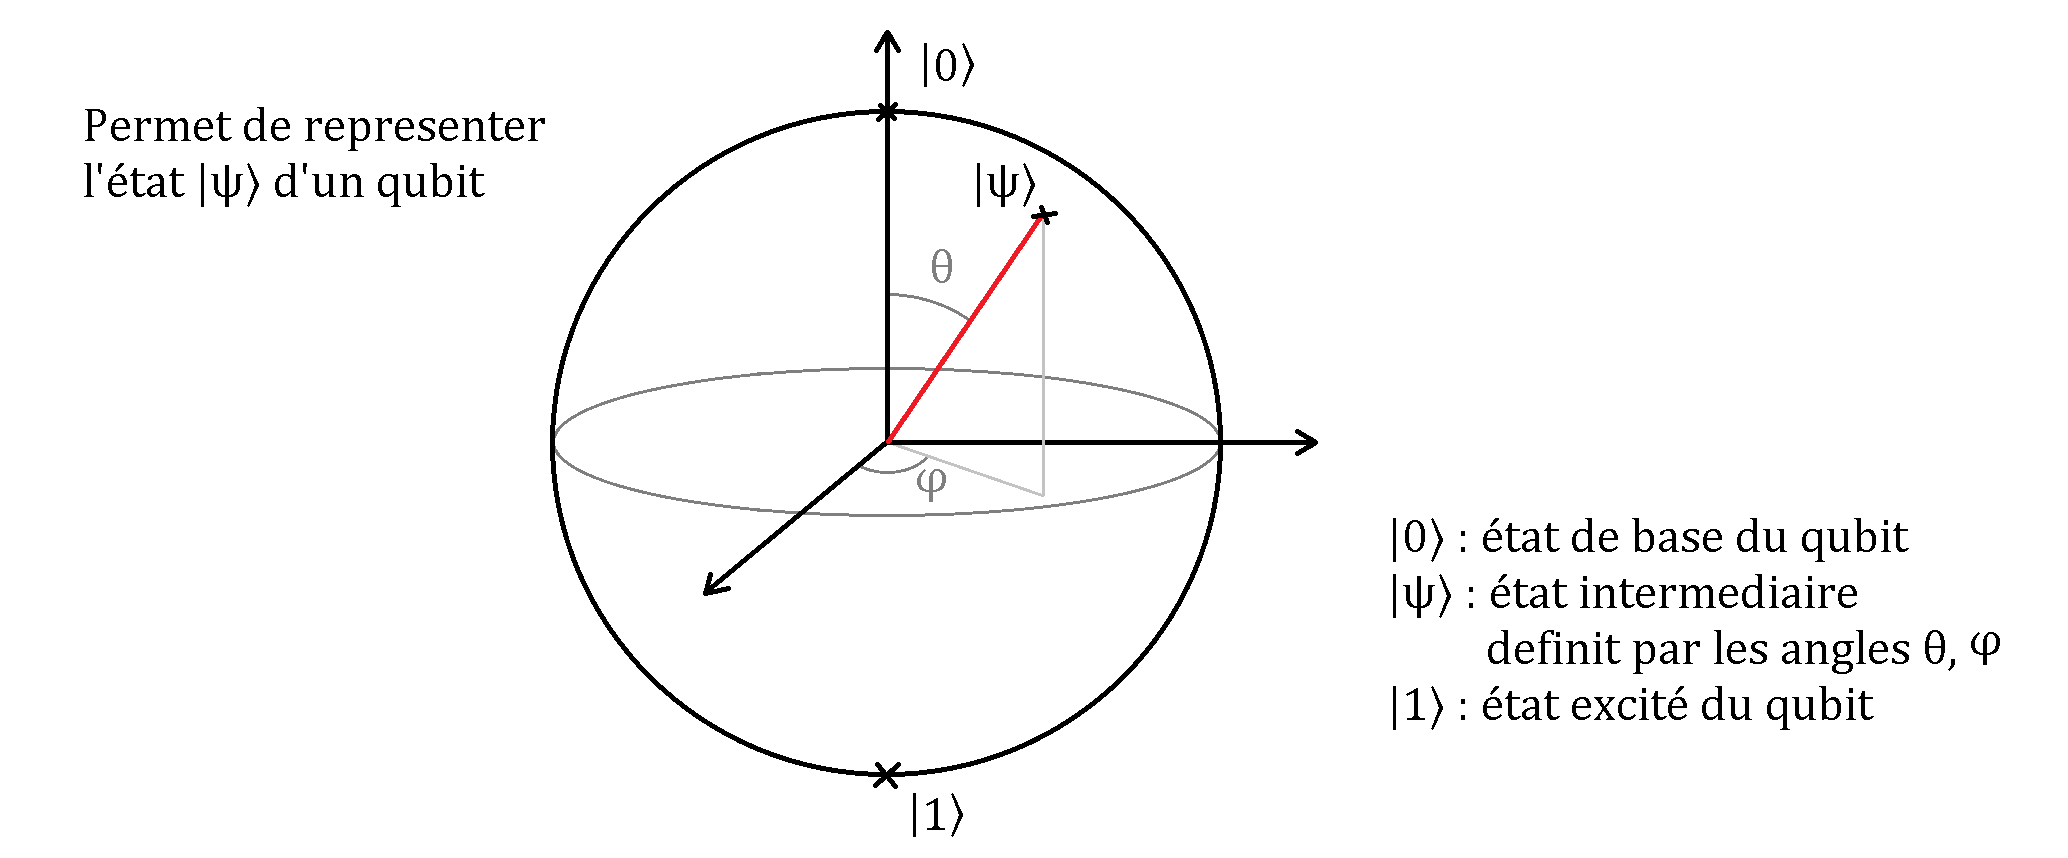
\includegraphics[scale=0.24]{sphere de boch.png}
 \centering
 \end{figure}

\begin{tabbing}
    On pose $\qquad R_x = \rho_{12} + \rho_{21} \qquad R_y = i(\rho_{21} - \rho_{12}) \qquad R_z = \rho_{22} - \rho_{11} = P_2 - P_1$.
\end{tabbing}

Relation entre $\Vec{R}$ et $\rho$ : $\qquad
\begin{cases}
    \rho(t) = \frac{1}{2}(I + \Vec{R}(t).\Vec{\sigma})\\
    R_i = Tr(\rho \sigma_i)
\end{cases}$

\begin{tabbing}
     Nous avons donc $R_z = \rho_{22} - \rho_{11} = P_2 - P_1 \qquad $ et $\qquad P_1 + P_2 = 1 = \rho_{11} + \rho_{22}$.\\
     $\Rightarrow \rho_{11} = 1 - \rho_{22} \Rightarrow R_z = 2\rho_{22} - 1 \Rightarrow \rho_{22} = \frac{1}{2} (1 + R_z)$.\\
     De même  $\rho_{11} = \frac{1}{2} (1 - R_z)$.\\
     Toutes les probabilités du système sont donc contenues dans la composante $R_z$.
\end{tabbing}


\newpage

\subsubsection{Description théorique}
Revenons à l'effet Zénon.\\
À $t=0$, nous allons nous poser au niveau 1 $\ket{1}$.\\
Comme dit précédemment, seuls deux états $\ket{1},\ket{2}$ sont accessibles dans le temps si on ne fait rien (décrit par l'équation de Schrödinger),\\
donc l'Hamiltonien de l'atome couplé au champ de radiofréquence est de dimension $2 \times 2$ et sur la base $(\ket{1},\ket{2})$ il a comme forme :

\begin{tabbing}
    \qquad $\hat H(t) = \frac{\hbar}{2} \begin{pmatrix}
\omega_0  & \Omega e^{-i\omega t} \\
\Omega e^{i\omega t}  & - \omega_0 
\end{pmatrix}$
\end{tabbing}

avec $\omega$ la pulsation du champ de radiofréquence. \\
\vspace{0.2cm}
Nous pouvons obtenir ce type d'Hamiltonien avec un certain champ magnétique \hyperref[sec:B]{\texttt{[1]}} par exemple.

\begin{tabbing}
    \quad $\hat H(t) = \frac{\hbar}{2} \Vec{H}.\Vec{\sigma}$ \quad donc $\Vec{H} = (\Omega \cos(\omega t), \Omega \sin(\omega t), \omega_0)$ \quad car les composantes sont $\frac{1}{\hbar} \text{Tr}(H\sigma_i)$
\end{tabbing}

avec $\hat{\Vec{\sigma}} = \begin{pmatrix}
\hat \sigma_x  \\
\hat \sigma_y \\
\hat \sigma_z
\end{pmatrix}$ où les $\hat \sigma_i$ correspondent aux matrices de Pauli.

Avec l'équation de Liouville \hyperref[sec:Liouville]{\texttt{[2]}}, on trouve :

\begin{tabbing}
    \qquad $\frac{d\Vec{R}}{dt} = \Vec{H}\times \Vec{R}$
\end{tabbing}

Ici, l'équation est compliquée à résoudre, si l'on prend un référentiel $Ox'y'z$ tournant à la pulsation $\omega$ autour de $Oz$ par rapport au référentiel $Oxyz$.

Dans le référentiel $Ox'y'z$, nous allons avoir :

\vspace{0.5cm}

\qquad $\rho'(t) = \hat U^\dagger(t) \rho(t) \hat U(t)$ \quad avec \quad $\hat U(t) = \begin{pmatrix}
e^{\frac{-i\omega t}{2}}  & 0 \\
0  & e^{\frac{i\omega t}{2}}
\end{pmatrix} = e^{-i\frac{\omega t}{2}\sigma_z}$

\vspace{0.4cm}

que nous allons poser comme définition de ce changement de référentiel.\\
\vspace{0.3cm}
Nous avons maintenant : $\frac{d\Vec{R'}}{dt} = \Vec{H'}\times \Vec{R'}$ avec $\Vec{H'} = (\Omega, 0, \omega_0 - \omega)$ car $\hat H'(t) = \frac{\hbar}{2} \Vec{H'}.\Vec{\sigma'}$.

\vspace{0.5cm}

Donc,

\[
\frac{d\Vec{R'}}{dt} = \begin{pmatrix}
    \Omega \\ 0\\0
\end{pmatrix} \times \begin{pmatrix}
    R_x' \\ R_y'\\R'_z
\end{pmatrix} = \begin{pmatrix}
    0 \\ -\Omega R'_z\\ \Omega R'_y
\end{pmatrix} = \begin{pmatrix}
    \dot{R}'_x \\ \dot{R}'_y\\\dot{R}'_z
\end{pmatrix}
\Rightarrow
\begin{cases}
    R'_z = -\cos(\Omega t)\\
    R'_y = \sin(\Omega t)
\end{cases}
\]

Nous allons, comme le protocole l'indique, mesurer à tout instant $t_n = \frac{\pi}{\Omega n} \Rightarrow R' = (0, 0, -\cos(\frac{\pi}{n}))$. Au bout de $N$ mesures, le vecteur $R'$ pointe dans la même direction qu'au départ mais la longueur est réduite d'un facteur $\cos(\frac{\pi}{N})^N$.

\vspace{0.5cm}

On a donc après $N$ mesures : $R'_z = -\cos(\frac{\pi}{N})^N$.\\
\vspace{0.3Cm}
Or avec ce changement de référentiel, nous avons $R'_z = R_z$.

\vspace{0.3cm}

Et précédemment, nous avions $\rho_{22} = \frac{1}{2} (1 + R_z) = P_2$. \\
\vspace{0.2cm}
Donc comme \qquad $P_2 = \frac{1}{2} (1 -\cos(\frac{\pi}{N})^N) \xrightarrow[N \rightarrow +\infty]{} 0$ \qquad et\qquad $P_1 \xrightarrow[N \rightarrow +\infty]{} 1$, \\
\vspace{0.3cm}
on a ici une démonstration théorique de l'effet Zénon :\\
si on mesure en continu l'état de notre système, l'état reste dans le même état.


\newpage

\subsubsection{Résultats expérimentaux}
\qquad Enfin, après avoir étudié la théorie, l'effet Zénon ne s'applique-t-il qu'à cette simple théorie ou a-t-il des effets dans la pratique ? Une expérience a été réalisée~\cite{exp}, en suivant la proposition de Cook, voici comment ils ont procédé :

\qquad Environ 5000 ions de béryllium ont été piégés dans un dispositif de Piège de Penning cylindrique, accompagnés d'ions de magnésium pour le refroidissement laser. Un laser continu à colorant de 313 nm a été utilisé pour exciter et détecter les transitions quantiques des ions de béryllium. Après avoir préparé les ions dans un état spécifique, des impulsions radiofréquences ont été appliquées pour manipuler leurs états quantiques. La fluorescence des ions de béryllium après chaque manipulation a été mesurée pour analyser les résultats.

\qquad Les résultats de l'expérience (voir figure 7) sont clairs : plus on augmente le nombre de mesures, plus la probabilité que notre système soit mesuré dans l'état $\ket{2}$ est proche de 0, comme on peut le voir sur le graphique :


\begin{figure}[h]
    \caption{Graphiques experimentales et théoriques, de la probabilité d'avoir la transition $1 \leftrightarrow 2$ ($p_2$) en fonction du nombre de pulse/mesure}
    \begin{subfigure}{0.5\textwidth}
        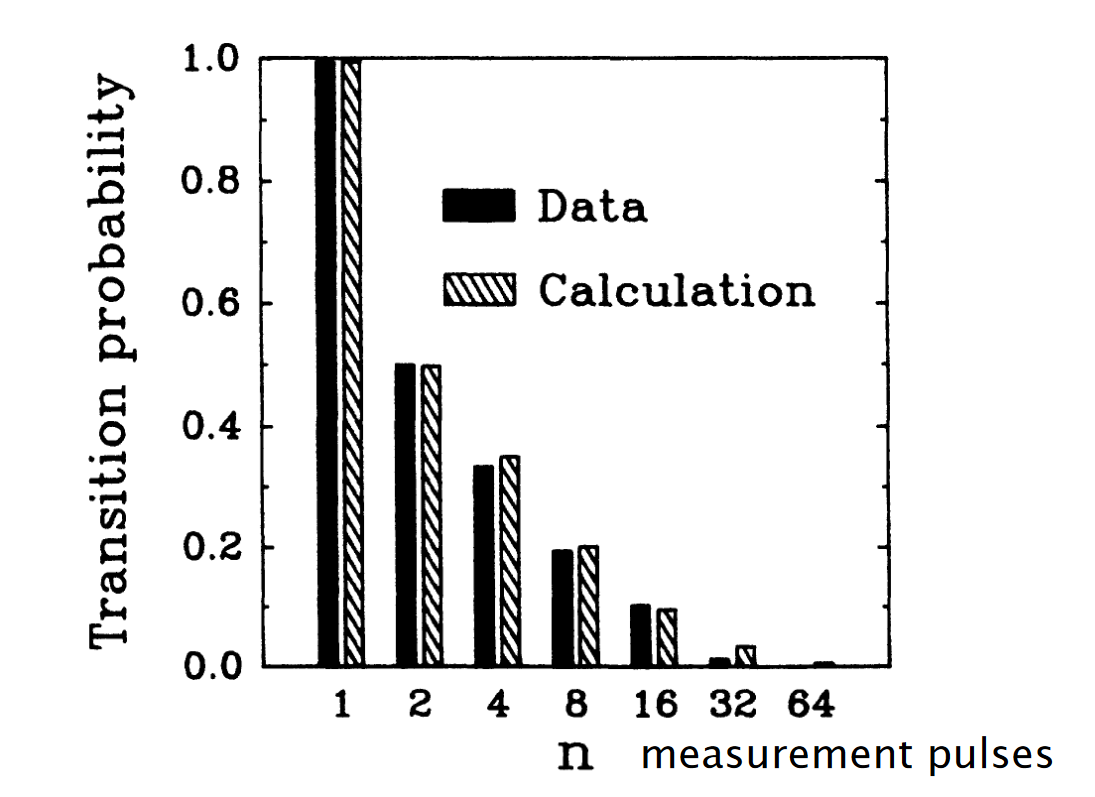
\includegraphics[scale=0.4]{graphe1.png}
        \caption{\label{transition12}Sens de la transition : $1 \rightarrow 2$ }
    \end{subfigure}
    \begin{subfigure}{0.5\textwidth}
        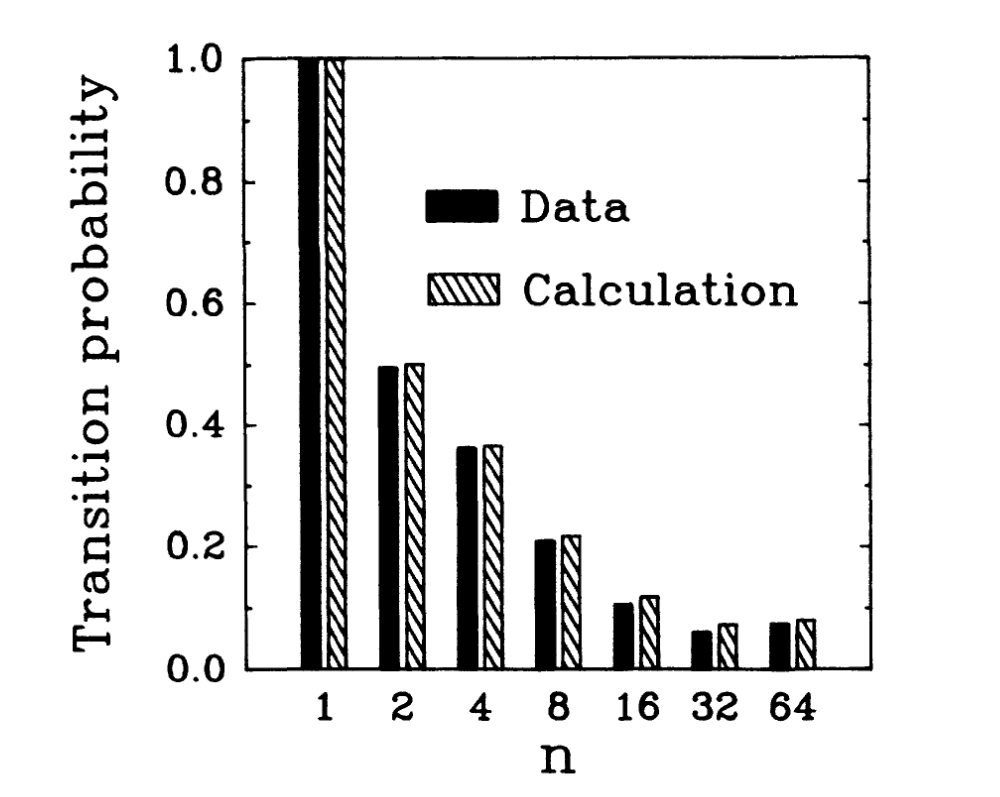
\includegraphics[scale=0.4]{graphe2.png}
        \caption{\label{transition21}Sens de la transition : $2 \rightarrow 1$}
    \end{subfigure}
\label{graphe experience}
\end{figure}

\vspace{0.3cm}

data = résultats de l'expérience\\
calculation = résultats théoriques\\

\vspace{0.5cm}

\qquad Le 2\textsuperscript{ème} graphique présente une augmentation pour 64 mesures due à un autre phénomène discuté dans l'article de l'expérience.

\vspace{1cm}

\qquad Tout cela nous permet bien d'affirmer l'existence de l'effet Zénon, que ce soit dans la théorie ou dans la pratique. Cet effet pourra être incontournable dans des domaines tels que l'informatique quantique où conserver l'état d'un qubit dans le temps est nécessaire pour éviter les erreurs. \\
\qquad Cela permettrait également au chat de Schrödinger de rester en vie dans la boîte ; en regardant continuellement l'atome, celui-ci ne changerait pas d'état et donc le poison ne pourrait pas se déclencher.


\newpage

\section{Conclusion}

\qquad En conclusion, j'ai pu apprendre pourquoi l'effet Zénon suggère que si un système quantique est observé en permanence, son évolution ou sa transition vers un état quantique différent peut être ralentie, voire arrêtée. Cela se produit parce que l’acte de mesure ou d’observation effondre l’état quantique en un résultat précis, empêchant le système d'explorer d'autres possibilités.\\
\vspace{0.3cm}
\qquad Ce stage a été une expérience enrichissante qui m'a permis d'explorer de manière approfondie la mesure quantique et l'effet Zénon. Il m'a également permis de réaliser à quel point la recherche dans ce domaine me passionne véritablement. De plus, la découverte et l'apprentissage du langage LaTeX ont été des compétences supplémentaires que j'ai acquises au cours de ce stage, élargissant ainsi mon parcours académique.\\
\vspace{0.3cm}
\qquad Bien que j'aurais aimé avoir plus de temps pour approfondir certains aspects, notamment en réalisant une approche numérique du phénomène étudié, je suis reconnaissant d'avoir eu l'opportunité d'explorer ces concepts fascinants.\\
\vspace{0.3cm}
\qquad Je tiens à exprimer ma gratitude envers mon maître de stage, Monsieur Fratino, pour m'avoir confié un sujet aussi captivant, qui correspond parfaitement à mes aspirations professionnelles. Son soutien et ses conseils tout au long de ce stage ont été précieux. \\
Je remercie également mon camarade A. Lefebvre avec qui j'ai partagé les recherches et qui m'a permis de rester motivé et travailleur tout au long de mon stage.



\newpage

\begin{thebibliography}{MMM99}

\bibitem[PstQ]{wikPM} Wikipedia, \href{https://fr.wikipedia.org/wiki/Postulats_de_la_m%C3%A9canique_quantique}{Postulat de la mécanique Quantique}\\

\bibitem[Prblm]{wikPRBLM} Wikipedia, \href{https://fr.wikipedia.org/wiki/Probl%C3%A8me_de_la_mesure_quantique}{Problème de la mesure quantique}\\

\bibitem[Red]{wikRED} Wikipedia, \href{https://fr.wikipedia.org/wiki/R%C3%A9duction_du_paquet_d'onde}{Réduction du paquet d'onde}\\

\bibitem[DecQ]{wikDQ} Wikipedia, \href{https://fr.wikipedia.org/wiki/D%C3%A9coh%C3%A9rence_quantique}{Décohérence quantique} \\

\bibitem[Fble]{wikF} Wikipedia, \href{https://fr.wikipedia.org/wiki/Mesure_faible}{Mesure faible}\\

\bibitem[QDupr]{Duprey} Thèse de Quentin Duprey sur \href{https://theses.hal.science/tel-02372565}{Mesure faible, Valeur Faible et Interférométrie}\\

\bibitem[DLou]{ColemanInt} Science étonante, \href{https://scienceetonnante.com/2022/12/08/mesure-quantique-coleman/}{Le problème de la mesure existe-t-il vraiment en mécanique quantique ?}\\

\bibitem[CK]{cook} \href{https://iopscience.iop.org/article/10.1088/0031-8949/1988/T21/009/meta}{Richard J Cook, What are Quantum Jumps?}
\bibitem[EKil]{ths} Thèse de Eva Kilian sur \href{https://homepage.univie.ac.at/reinhold.bertlmann/pdfs/dipl_diss/EvaKilian_BA_QuantumZenoEffect_Interaction-freeMeasurements.pdf}{Interaction-free Measurements}\\

\bibitem[MQ2]{livre} \textit{Mécanique Quantique 2, Développements et applications a basse énergie 4ème édition} de C. Aslangul, Page 1005-1024\\

\bibitem[RabCle]{wik6} Wikipedia, \href{https://en.wikipedia.org/wiki/Rabi_cycle}{Rabi cycle}\\

\bibitem[VcRab]{wik12} wikipedia, \href{https://en.wikipedia.org/wiki/Jaynes%E2%80%93Cummings_model#Vacuum_Rabi_oscillations}{Jaynes Cummings model Vacuum Rabi oscillations}\\

\bibitem[Gui]{G} Guillod, \href{https://guillod.org/teaching/mecanique-quantique1/Cours-systeme-2niveaux.pdf}{Systèmes à deux niveaux}\\

\bibitem[Ujf]{stat} Ujf-grenoble, \href{https://www-fourier.ujf-grenoble.fr/~faure/enseignement/meca_q/cours_chap9.pdf}{Statistiques quantiques}\\

\bibitem[It]{exp} Experience et Théorie de l'effet Zénon, \href{https://goldphysics.unm.edu/phys521/features/zeno_PhsRevA41_2299.pdf}{article de Wayne M. Itano, D. J. Heinzen, J. J. Bollinger, et D. J. Wineland}\\

\bibitem[EttQ]{wik45} Wikipedia, \href{https://fr.wikipedia.org/wiki/%C3%89tat_quantique}{état quantique}\\

\bibitem[BlchS]{wikBLC} Wikipedia, \href{https://en.wikipedia.org/wiki/Bloch_sphere}{Bloch sphere}
\\
\vspace{0.7cm}
\bibitem[FGR]{figure}Figure faites par mes soins
\end{thebibliography}

\newpage

\section{Annexe}

{\texttt{[1]}}\label{sec:B} Demonstration de l'utilisation d'un champs magnétique~\cite{G} pour trouver l'Hamiltonien d'un atome couplé au champs de radifrequence :\\
\vspace{0.3cm}
si on prend un champs magnétique :
\begin{tabbing}
    \qquad $\Vec{B}(t) = \begin{pmatrix}
B_1 cos(\omega t)  \\
B_1 sin(\omega t) \\
B_0
\end{pmatrix}$ 
\end{tabbing}

L'hamiltonien dans un champ magnétique $\Vec{B}(t)$ est :\\
\begin{tabbing}
    \qquad \= $\hat H(t) = - \mu B = - \gamma \Vec{B}(t).\hat{\Vec{S}}$
\end{tabbing}

avec $\hat{\Vec{S}} = \frac{\hbar}{2} \begin{pmatrix}
\hat \sigma_x  \\
\hat \sigma_y \\
\hat \sigma_z
\end{pmatrix}$ où les $\hat \sigma_i$ correspondent aux matrices de Pauli

\begin{tabbing}
on a donc $\hat H(t) = \frac{\hbar}{2}(- \gamma B_1 cos(\omega t) \hat \sigma_x - \gamma B_1 sin(\omega t) \hat \sigma_y - \gamma B_0 \hat \sigma_z) = \frac{\hbar}{2} \begin{pmatrix}
- \gamma B_0  & - \gamma B_1 e^{-i\omega t} \\
- \gamma B_1 e^{i\omega t}  & + \gamma B_0 
\end{pmatrix}$
\end{tabbing}

Soient $\omega_0 = - \gamma B_0$ et $\omega_1 = - \gamma B_1$\\
si l'on pose notre champs magnétique tels que  $\omega_1 = \Omega = \sqrt{(\omega-\omega_0)^2+\omega_1^2}$ la frequence de Rabi et donc $\omega = \omega_0 $ la frequence de raisonnace.

\begin{tabbing}
    on obtient donc $\hat H(t) = \frac{\hbar}{2} \begin{pmatrix}
\omega_0  & \Omega e^{-i\omega t} \\
\Omega e^{i\omega t}  & - \omega_0 
\end{pmatrix}$
\end{tabbing}
\vspace{0.5cm}

%%%%%%%%%%%%%%%%%%%%%%%%%%%%%
{\texttt{[2]}} \label{sec:Liouville}Demonstration de l'utilisation de Liouville pour avoir l'equation Gyroscopique :
\begin{tabbing}
    l'équation de Liouville en quantique s'écrit : $\qquad i\hbar \frac{\partial \rho}{\partial t} = [H, \rho]$
\end{tabbing}

\begin{tabbing}
    et $\qquad \hat H(t) = \frac{\hbar}{2} \Vec{H}.\Vec{\sigma}, \qquad \rho = \frac{1}{2}(I + \Vec{R}.\Vec{\sigma})$
\end{tabbing}
donc
\begin{flalign}
    \qquad i\hbar \frac{\partial \rho}{\partial t} & = [\frac{\hbar}{2} \Vec{H}.        \Vec{\sigma}, \frac{1}{2}(I + \Vec{R}.\Vec{\sigma})] & \\
    & = \frac{\hbar}{4}[ \Vec{H}.\Vec{\sigma}, (I + \Vec{R}.\Vec{\sigma})] &\\
    & = \frac{\hbar}{4}([ \Vec{H}.\Vec{\sigma},I] + [\Vec{H}.\Vec{\sigma},\Vec{R}.\Vec{\sigma}])&\\
    & = \frac{\hbar}{4}[\Vec{H}.\Vec{\sigma},\Vec{R}.\Vec{\sigma}]&
\end{flalign}
D'autre part 
\begin{flalign}
    \qquad i\hbar \frac{\partial \rho}{\partial t} & = i \hbar \frac{d}{dt}(\frac{1}{2}(I +\Vec{R}.\Vec{\sigma})&\\
    & =  \frac{i \hbar}{2} \frac{d\Vec{R}}{dt}.\Vec{\sigma}&
\end{flalign}
donc $\qquad \frac{i \hbar}{2} \frac{d\Vec{R}}{dt}.\Vec{\sigma} =  \frac{\hbar}{4}[\Vec{H}.\Vec{\sigma},\Vec{R}.\Vec{\sigma}] = \frac{\hbar}{4} ((\Vec{H}.\Vec{\sigma})(\Vec{R}.\Vec{\sigma}) - (\Vec{R}.\Vec{\sigma})(\Vec{H}.\Vec{\sigma}))$
\begin{tabbing}
    or nous posons l'égalité suivante comme vrai ici~\cite{livre} : $(\Vec{\sigma}.\Vec{A})(\Vec{\sigma}.\Vec{B}) = \Vec{A}.\Vec{B}I + i \Vec{\sigma}.(\Vec{A}\times \Vec{B})$
\end{tabbing}
donc 
\begin{flalign}
    \qquad i \frac{d\Vec{R}}{dt}.\Vec{\sigma} & = \frac{1}{2} (\Vec{H}.\Vec{R}I + i \Vec{\sigma}.(\Vec{H}\times \Vec{R}) - \Vec{R}.\Vec{H}I - i \Vec{\sigma}.(\Vec{R}\times \Vec{H}))&\\
    & = \frac{1}{2} (2i \Vec{\sigma}.(\Vec{H}\times \Vec{R})) &
\end{flalign}
$\qquad \qquad \Leftrightarrow \frac{d\Vec{R}}{dt} = \Vec{H}\times \Vec{R} \qquad \leftarrow\qquad $ l'équation "gyroscopique"


\end{document}           

\newpage
Diagonalisation de la matrice \( \hat{H}(t) \) :\\
\vspace{0.5cm}
La matrice \( \hat{H}(t) \) est donnée par :

\[
\hat{H}(t) = \frac{\hbar}{2} \begin{pmatrix}
\omega_0 & \Omega e^{-i\omega t} \\
\Omega e^{i\omega t} & - \omega_0
\end{pmatrix}
\]

Pour trouver les valeurs propres \( \lambda_{\pm} \), nous devons résoudre l'équation caractéristique :

\[
\text{Det}(\hat{H}(t) - \lambda I) = 0
\]
Les valeurs propres de l'Hamiltonien sont donc :\\
\vspace{0.5cm}
$\lambda_+ = \frac{\hbar}{2} \sqrt{\omega_0^2 + \Omega^2},$\qquad$\lambda_- = -\frac{\hbar}{2} \sqrt{\omega_0^2 + \Omega^2}.$\\
\vspace{1cm}

Les vecteurs propres correspondants sont :\\
\vspace{0.5cm}
Pour \(\lambda_+ \):
\[ \vec{v_+} = \begin{pmatrix} \frac{\omega_0 + \sqrt{\omega_0^2 + \Omega^2}}{\Omega} e^{-i\omega t} \\ 1 \end{pmatrix} \]
Pour \(\lambda_-\):
\[ \vec{v_-} = \begin{pmatrix} -\frac{\sqrt{\omega_0^2 + \Omega^2}-\omega_0 }{\Omega} e^{-i\omega t} \\ 1 \end{pmatrix} \]
Résultat trouvé avec \href{https://www.dcode.fr/vecteurs-propres-matrice}{dcode} car le système etait trop compliqué...
